\ifx\mainfile\undefined
%  ========================================================================
%  Copyright (c) 2006-2011 The University of Washington
%
%  Licensed under the Apache License, Version 2.0 (the "License");
%  you may not use this file except in compliance with the License.
%  You may obtain a copy of the License at
%
%      http://www.apache.org/licenses/LICENSE-2.0
%
%  Unless required by applicable law or agreed to in writing, software
%  distributed under the License is distributed on an "AS IS" BASIS,
%  WITHOUT WARRANTIES OR CONDITIONS OF ANY KIND, either express or implied.
%  See the License for the specific language governing permissions and
%  limitations under the License.
%  ========================================================================
%
 
\documentclass [11pt, twoside] {uwthesis}

\usepackage{color}
\usepackage{url}
\usepackage{amsmath}
\usepackage{amsfonts}
\usepackage[bookmarks,
	hidelinks,
	plainpages=false,
	pdfpagelabels,
	pagebackref=true,
            ]{hyperref}
\renewcommand*{\backref}[1]{}% for backref < 1.33 necessary
\renewcommand*{\backrefalt}[4]{%
  \ifcase #1 %
    (No citations.)%
  \or
    (Cited on page #2.)%
  \else
    (Cited on pages #2.)%
  \fi
}

\newcommand{\biburl}[1]{{\tt<}\url{#1}{\tt>}}

\hypersetup{%
pdfauthor = {Daniel Chaim Halperin},
pdftitle = {Simplifying the Configuration of 802.11 Wireless Networks with Effective SNR},
pdfsubject = {Ph.D. Dissertation},
pdfkeywords = {},
pdfcreator = {University of Washington, Computer Science and Engineering},
pdfproducer = {},
bookmarksopen = {true},
pdfpagelayout = {TwoColumnRight},
}

\usepackage{footnotebackref}
%%%%%%%%%%%%%%%%%%%%%%%%%%%%%%%%%%%%%%%%%%%%%%%%%%%%%%
%%%        Formatting sections                     %%%
%%%%%%%%%%%%%%%%%%%%%%%%%%%%%%%%%%%%%%%%%%%%%%%%%%%%%%
\newcommand{\algref}[1]{Algorithm~\ref{#1}}
\newcommand{\chapref}[1]{Chapter~\ref{#1}}
\renewcommand{\eqref}[1]{Equation~\ref{#1}}
\newcommand{\figref}[1]{Figure~\ref{#1}}
\newcommand{\secref}[1]{\S\ref{#1}}
\newcommand{\tabref}[1]{Table~\ref{#1}}
\newcommand{\heading}[1]{\vspace{4pt}\noindent\textbf{#1}}
\newcommand{\topheading}[1]{\noindent\textbf{#1}}
\newcommand{\noheading}[0]{\vspace{4pt}\noindent}

%%%%%%%%%%%%%%%%%%%%%%%%%%%%%%%%%%%%%%%%%%%%%%%%%%%%%%
%%%        XXX and other warnings                  %%%
%%%%%%%%%%%%%%%%%%%%%%%%%%%%%%%%%%%%%%%%%%%%%%%%%%%%%%
\newcommand{\xxx}[1]{\textit{\color{red}XXX #1}}

%%%%%%%%%%%%%%%%%%%%%%%%%%%%%%%%%%%%%%%%%%%%%%%%%%%%%%
%%%        Units                                   %%%
%%%%%%%%%%%%%%%%%%%%%%%%%%%%%%%%%%%%%%%%%%%%%%%%%%%%%%
\usepackage{xspace}
\newcommand{\unitsep}{\texorpdfstring{\,}{ }}
\def\unit#1{% from: http://www.tex.ac.uk/cgi-bin/texfaq2html?label=csname "Defining a macro from an argument"
  \expandafter\def\csname #1\endcsname{\unitsep\text{#1}\xspace}%
}
\def\varunit#1#2{% from: http://www.tex.ac.uk/cgi-bin/texfaq2html?label=csname "Defining a macro from an argument"
  \expandafter\def\csname #1\endcsname{\unitsep\text{#2}\xspace}%
}
\unit{GHz}
\unit{MHz}
\unit{kHz}
\unit{Gbps}
\unit{Mbps}
\unit{KB}
\unit{dB}
\unit{dBi}
\unit{dBm}
\unit{W}
\unit{mW}
\varunit{uW}{$\mu$W}
\unit{ms}
\varunit{us}{$\mu$s}
\unit{h}
\unit{m}
\unit{s}
\unit{km}
\unit{cm}
\unit{mm}
\varunit{mmsq}{mm$^\text{2}$}
\varunit{insq}{in$^\text{2}$}
\newcommand{\degree}{\ensuremath{^\circ}\xspace}
\newcommand{\degrees}{\degree}
%%%%%%%%%%%%%%%%%%%%%%%%%%%%%%%%%%%%%%%%%%%%%%%%%%%%%%%%%%%%%%%%%%%%%%%%%%%%%%%%%%%%%%
% Euler for math | Palatino for rm | Helvetica for ss | Courier for tt
%
% From: http://www.tug.org/mactex/fonts/LaTeX_Preamble-Font_Choices.html
%%%%%%%%%%%%%%%%%%%%%%%%%%%%%%%%%%%%%%%%%%%%%%%%%%%%%%%%%%%%%%%%%%%%%%%%%%%%%%%%%%%%%%
\renewcommand{\rmdefault}{ppl} % rm
\usepackage[scaled]{helvet} % ss
\usepackage{courier} % tt
\usepackage{eulervm} % a better implementation of the euler package (not in gwTeX)
\normalfont
\usepackage[T1]{fontenc}
%%%%%%%%%%%%%%%%%%%%%%%%%%%%%%%%%%%%%%%%%%%%%%%%%%%%%%%%%%%%%%%%%%%%%%%%%%%%%%%%%%%%%%

%%%%%%%%%%%%%%%%%%%%%%%%%%%%%%%%%%%%%%%%%%%%%%%%%%%%%%
%%%        Figures                                 %%%
%%%%%%%%%%%%%%%%%%%%%%%%%%%%%%%%%%%%%%%%%%%%%%%%%%%%%%
\usepackage{graphicx}
% Caption package both lets you set the spacing between figure and caption
% and also makes the \figref{} point to the right place.
\usepackage[font=bf,aboveskip=6pt,belowskip=-4mm]{caption}
% Allow subfigures, make them bold
\usepackage[bf,BF,small]{subfigure}
% List of figures
\setcounter{lofdepth}{2}  % Print the chapter and sections to the lot

%%%%%%%%%%%%%%%%%%%%%%%%%%%%%%%%%%%%%%%%%%%%%%%%%%%%%%
%%%        Lists with reduced spacing              %%%
%%%%%%%%%%%%%%%%%%%%%%%%%%%%%%%%%%%%%%%%%%%%%%%%%%%%%%
\usepackage{enumitem}

%%%%%%%%%%%%%%%%%%%%%%%%%%%%%%%%%%%%%%%%%%%%%%%%%%%%%%
%%%        Fancy tables                            %%%
%%%%%%%%%%%%%%%%%%%%%%%%%%%%%%%%%%%%%%%%%%%%%%%%%%%%%%
\usepackage{tabulary}
\usepackage{booktabs}

%%%%%%%%%%%%%%%%%%%%%%%%%%%%%%%%%%%%%%%%%%%%%%%%%%%%%%
%%%        Formatting techniques/tools/etc.        %%%
%%%%%%%%%%%%%%%%%%%%%%%%%%%%%%%%%%%%%%%%%%%%%%%%%%%%%%
\newcommand{\term}[1]{\texttt{#1}}

\begin{document}
 
\textpages
\setcounter{chapter}{5} % Set to n-1!
\fi
%%%%%%%%%%%%%%%%%%%%%%%%%%%%%%%%%%

\cleardoublepage
\chapter{Packet Delivery over MIMO Channels}
\label{chap:delivery}

In this chapter, I experimentally evaluate how well my Effective SNR model predicts packet delivery for 802.11n wireless links. This is the fundamental measure of whether the model can be useful; good predictions are necessary to properly configure links and networks to solve the link and network configuration problems.

To do so, I use my CSI measurement tool to gather a wide range of channel and performance information across 200 wireless links in both testbeds. This captures a wide variety of fading environments, from line-of-sight links in the same room to links between nodes in different rooms with RF barriers and reflectors spread around and between them. I then use this data to evaluate the accuracy of predictions made when using Packet SNR and Effective SNR about whether packets will be delivered.

\section{Experimental Data}
I measured packet delivery over a 20\MHz channel on my two 802.11n testbeds, using links with four different antenna configurations:
\begin{enumerate}
\item The \textbf{SISO} configuration uses a single antenna at each node. This configuration corresponds to 802.11a.
\item The \textbf{SIMO} configuration uses a single transmit antenna but three receive antennas. This is an 802.11a/g/n configuration that uses spatial diversity techniques.
\item The \textbf{MIMO2} configuration uses two spatial streams and three receive antennas. This employs both 802.11n techniques of spatial multiplexing and spatial diversity.
\item The \textbf{MIMO3} configuration uses three antennas at each node to send and receive three spatial streams. This configuration uses spatial multiplexing, but does not additionally benefit from spatial diversity.
\end{enumerate}

For each of these configurations, I measured the packet delivery for each link using each MCS, at at each transmit power level between $-$10\dBm and $+$16\dBm in steps of 2\dB. I sent 1,500-byte packets as constant bit-rate UDP traffic generated by \program{iperf} at 2\Mbps for 5 seconds, about 860 packets total. The receiver also recorded the CSI and per antenna RSSIs and noise floors to measure the RF channel for each correctly received packet. In these experiments, I turned off 802.11's link layer retransmissions in order to observe the underlying packet delivery rate. The experiments were conducted at night on unused 802.11 channels in order to minimize the effects of environmental movement and RF interference on these results.

%Note that CSI and RSSI are measured during the preamble, and so do not depend on the transmit rate, though they vary with the number of streams. 
%Similarly, 3x3 CSI gives us the channel between each pair of transmit and receive antennas, so it also implicitly contains 1x1 CSI\@.

The above testing gives ground truth data to probe variation across 200 links, 26\dB of transmit power, four antenna configurations ranging from SISO to MIMO3, and 8 MCS values per configuration. This covers all of the key variables needed to implement and evaluate my Effective SNR model. 

\section{Computing SNR}
Using these measurements, I computed the packet reception rate (PRR), Packet SNR, and Effective SNRs for all the measured configurations.

\subsection{Computing Packet SNR}
The natural 
When receiving a transmission with multiple antennas, there is one RSSI value per antenna; how should these measurements be combined into a single SNR value for the link? I first convert the per-antenna RSSI and noise measurements to SNRs (\eqref{eq:per_chain_snr}) and then sum the SNRs. This is a straightforward choice for a single spatial stream as it corresponds to receiver processing using maximal-ratio combining (\eqref{eq:mrc}). It is also reasonable for 2- and 3-stream MIMO because the symbols carried on different spatial streams are interleaved coded bits~\cite{80211n}.

\subsection{Computing Effective SNRs}
From these data, I compute Effective SNR values using the model described in \chapref{chap:model}. I parameterized the model using known properties of the Intel IWL5300 devices: they use minimum mean square error (MMSE) MIMO equalizers, and have known, fixed spatial mapping matrices.

\section{Results}
The goal of this chapter is to understand whether Effective SNR is a good metric, whether it is an accurate predictor of packet delivery. In this section, I evaluate this in two ways. The first is via the \define{transition window}, i.e., the SNR regime in which packet delivery for all links goes from near-zero to near-perfect. We saw in \chapref{chap:problem} that this transition occurs rapidly for a wired link (\figref{fig:snr_prr_attenuator}), but occurs over a wide range for wireless links (\figref{fig:snr_prr_26_65}) when using the Packet SNR. A narrow transition window would be one indicator that Effective SNR works well.

The second evaluation metric is \define{rate confusion}, i.e., how many rates might be best at a particular SNR value. The wired link showed clear separation between rates, such that at every SNR value there is a clear best rate. Conversely, because the transition regions of different wireless links overlap, links with the same Packet SNR might support very different rates. Here, I compare the degree of rate confusion between Packet SNR Effective SNR.

\subsection{Transition Windows}
\begin{table}
\centering
\begin{tabular}{cccccc}
\toprule
\multirow{2}{*}{MCS} & \multirow{2}{*}{Rate (Mbps)} & \multicolumn{2}{c}{$\Delta\rho_{\text{packet}}$ (dB)} &
\multicolumn{2}{c}{$\Delta\rho_{\text{eff}}$ (dB)} \\ 
\cmidrule(lr){3-4} \cmidrule(lr){5-6}
& &  ~~5\%--95\% & ~25\%--75\% & ~~5\%--95\% & ~25\%--75\%  \\
\midrule 
0 &  6.5                    & 3.08  & 1.29  & 2.05  & 0.81 \\
1 & 13.0                    & 3.45  & 1.44  & 2.38  & 0.89 \\
2 & 19.5                    & 6.27  & 3.12  & 2.30  & 0.85 \\
3 & 26.0                    & 3.93  & 1.98  & 3.02  & 0.94 \\
4 & 39.0                    & 7.05  & 3.49  & 2.19  & 0.93 \\
5 & 52.0                    & 7.16  & 3.20  & 2.29  & 1.06 \\
6 & 58.5                    & 7.25  & 3.37  & 2.92  & 1.41 \\
7 & 65.0                    & 7.24  & 2.81  & 2.92  & 1.35 \\
\midrule
\multicolumn{2}{c}{Average} & 5.68  & 2.59  & 2.51  & 1.03 \\         
\bottomrule
\end{tabular}
\caption{\label{tab:transitions} Width of SISO transition windows.}
\end{table}

I analyzed the SISO measurements to find the transition window for each of the measured links. I define the window to be the SNR values between which packet delivery rises from 10\% (lossy) to 90\% (reliable) for any link.

\tabref{tab:transitions} gives the width of the transition window (denoted $\Delta\rho$) for SISO rates using the Packet SNR and Effective SNR metrics. I show the 25\%--75\% range of points in the transition window as a measure of the typical link, and the 5\%--95\% range as a measure of most links. A good result here is a narrow window like that measured over a wire (\figref{fig:snr_prr_attenuator}).

The table shows that the transition widths are consistently tight with my model. Most links transition within a window of around 2\dB for most rates. The width of the SNR-based transition windows is typically two to three times looser, especially for the denser modulation schemes like 64-QAM and higher code rates. This means that it is easy for a less than ideal channel to degrade the reception of high rates. However, while the transitions for the last four rates are inflated with SNR, they remain tight with Effective SNR\@. 

The results for Effective SNR are in fact about the best that can be obtained because they are close to textbook transitions for flat-fading channels and those measured over a wire (\figref{fig:snr_prr_attenuator}). A small improvement is surely possible, but this is probably limited by the precision of my measurement data. The IWL5300 gives RSSI, AGC and noise values in dB to the nearest integer, and at most 8-bit CSI over a 48\dB range for 30 out of 56 subcarriers. With these factors, quantization error of at least 1\dB is likely.

The larger significance of narrow transition windows is that, by reducing them enough that they do not overlap, I can unambiguously predict the highest rate that will work for nearly all links nearly all of the time. In contrast, Packet SNR transition windows overlap such that for a given SNR there may be five different best rates across links the testbed. I explore this in the next section.


\subsection{Rate Confusion}
\label{sec:rate_confusion}

\begin{figure}[t]
	\centering
	\subfigure[SISO]{
		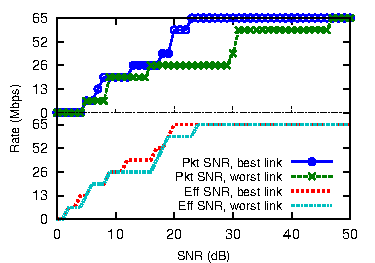
\includegraphics[width=0.49\textwidth, clip]{figures/esnr/embed_ratestep_snr_1x1_90.pdf}%
		\label{fig:snr_rate_step_1x1}%
	}\hfill%
	\subfigure[SIMO]{
		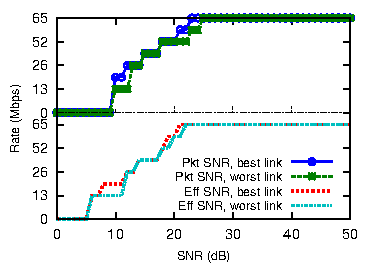
\includegraphics[width=0.49\textwidth, clip]{figures/esnr/embed_ratestep_snr_1x3_90.pdf}%
		\label{fig:snr_rate_step_1x3}%
	}
	
	\subfigure[MIMO2]{
		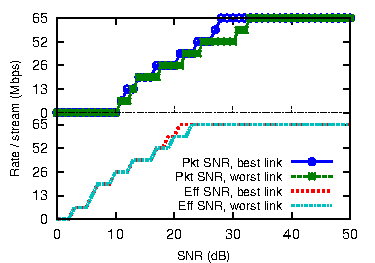
\includegraphics[width=0.49\textwidth, clip]{figures/esnr/embed_ratestep_snr_2x3_90.pdf}%
		\label{fig:snr_rate_step_2x3}%
	}\hfill%
	\subfigure[MIMO3]{
		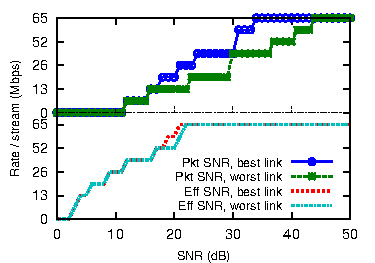
\includegraphics[width=0.49\textwidth, clip]{figures/esnr/embed_ratestep_snr_3x3_90.pdf}%
		\label{fig:snr_rate_step_3x3}%
	}
	\caption[The variation of best rate with SNR over links and antenna configurations]{\label{fig:snr_rate_steps}The variation of best rate with SNR over links and antenna configurations. Excepting extremely low and high SNRs, one RSSI-based packet SNR value maps to multiple best rates for different links, %. For the same data, 
while Effective SNR provides a clear indicator of the best rate for nearly all links.}
\end{figure}

To understand whether the Effective SNR model accurately predicts packet delivery, I analyze the fastest working rate (PRR$\geq$ 90\%) for each link and all NIC settings. \figref{fig:snr_rate_steps} shows the results broken down by configuration. The SISO experiment (\figref{fig:snr_rate_step_1x1}) shows links for both testbeds combined. The remaining graphs \figref{fig:snr_rate_step_1x3}--\ref{fig:snr_rate_step_3x3}  show rates for SIMO, MIMO2 and MIMO3 configurations for the Intel testbed only; it is denser than UW and supports MIMO experiments over our NIC's transmit power range.

These graphs study rate confusion, i.e., the ability of a given SNR value to predict the best rate across a wide set of links. If we consider the fastest rate each link supports at a particular Packet SNR or Effective SNR value, the best link is the link that supports the fastest rate, and the worst link is the slowest. The difference between the best and worst links, i.e., the set of possible best rates for an arbitrary link with a particular SNR, is the rate confusion. I plot this spread in these graphs. Note that the SIMO figure does not include data for the lowest 6.5\Mbps rate, because very few links experience loss at that rate within the transmit power range of the IWL5300---the added spatial diversity makes most links work well, as described below.

Ideally, the best and worst lines would overlap completely, such that the highest rate for a given SNR would be the same for the best and worst links. This rate would then be an accurate prediction for the particular Effective SNR or Packet SNR level. Conversely, gaps between the best and worst lines expose confusion about which rate will be the highest rate for that SNR.

For the SISO (\figref{fig:snr_rate_step_1x1}) and MIMO3 (\figref{fig:snr_rate_step_3x3}) cases, the figures show that using Packet SNR results in a large spread between the best and worst lines. Except for extremely low and high SNRs, nearly all SNRs have at least two---and up to five different---rates as suitable choices for the best rate. That is, Packet SNR often poorly indicates rate.

In sharp contrast, %looking at bottom lines in the graphs, 
the two Effective SNR lines overlap almost all the time, and mostly appear to be a single line. This is almost an ideal result. Effective SNR is a clear indicator of best rate. When there is slight separation, the spread is only between rates that use the same modulation but different amounts of coding. These combinations are also close together in our wired experiments. 

Interestingly, these results show that Packet SNR predictions are much better for the SIMO and MIMO3 cases, though still not as accurate as Effective SNR, particularly for the highest rates. The reason is \emph{spatial diversity}: spare receive antennas gather the received signal and combine to make the channel more frequency-flat, thus bringing the Packet SNR closer to the Effective SNR. This effect is well-known, though typically not observable using real 802.11 NICs which, except my prototype implementation, do not export CSI. This result suggests that Packet SNR \emph{is} a reasonable predictor for an 802.11 configuration with significant diversity. Still, observe that Packet SNR does not transfer well across the antenna modes (as diversity gains and inter-stream interference change unpredictably) which makes this less useful. This is one reason that SISO rate adaptation schemes do not translate to MIMO.

Finally, I note that neither Effective SNR nor Packet SNR performs extremely well at the lowest modulation at low SNRs. I believe this artifact arises from errors in the AGC values reported by the NIC, observed by Judd et al.~\cite{Judd_CHARM} and confirmed by my data for Intel's hardware.

\section{Summary}
From these results, I conclude that Effective SNR consistently and accurately indicates the best rate for nearly all links and all configurations without any per-link calibration. The low degree of rate confusion with Effective SNR in \secref{sec:rate_confusion} implies that it should be possible to define SNR thresholds that clearly define when a rate will work well. I discuss how to choose these thresholds in the next chapter,\footnote{\textcolor{red}{XXX: or, where should this be? It's not really necessary yet, not until we start making algorithmic choices.}} in which I deploy my Effective SNR as part of a system that selects the optimal rate for a wireless link.

\textcolor{red}{XXX Which reminds me: where should I mention quantization error?}
%From now on, we use the thresholds in these graphs to predict the working rate for any link. They agree with the measured SNRs on a wired link (\figref{fig:snr_prr_attenuator}), which strongly suggests that the Effective SNR captures the fundamental error characteristics of the link. 

\textcolor{red}{XXX include this?: We also demonstrate that the Effective SNR model enables a sender to accurately prune excess transmit power from a strong link while maintaining high packet delivery.}

%%%%%%%%%%%%%%%%%%%%%%%%%%%%%%%%%%
\ifx\mainfile\undefined
%
% ==========   Bibliography   ==========
%
%\nocite{*}   % include everything in the uwthesis.bib file
\bibliographystyle{plain}
\bibliography{dhalperi_thesis}

\end{document}
\fi
